\documentclass[12pt,reqno]{amsart}

\usepackage{amsthm,amsmath,amssymb}
\usepackage{mathtools}
\usepackage{proof}
\usepackage{centernot}
\usepackage{xcolor}
\usepackage{graphicx}
\usepackage[T1]{fontenc}
\usepackage{courier}
\usepackage{enumitem}
\usepackage{hyperref}
\usepackage{array}
\usepackage{multirow}
\usepackage{algorithmic}
\usepackage{textcomp}
\usepackage{algorithm}
\usepackage{cite}
\usepackage{listings}
\lstset{basicstyle=\ttfamily\tiny, columns=fullflexible, language=Python, morekeywords={logical_and, log, exp, dot, sqrt, ones, identity}}
\definecolor{mySucces}{RGB}{40, 167, 69}
\definecolor{myFail}{RGB}{220, 53, 69}

\newcommand{\code}[1]{\texttt{#1}}
\newcommand{\st}[0]{\text{ s.t. }}
\newcommand{\where}[0]{\text{ where }}
\newcommand{\mand}[0]{\text{ and }}
\newcommand{\msgspc}[0]{\mathcal{M}}
\newcommand{\cphspc}[0]{\mathcal{C}}
\newcommand{\keyspc}[0]{\mathcal{K}}
\newcommand{\advrs}[0]{\mathcal{A}}
\newcommand{\distin}[0]{\mathcal{D}}
\newcommand{\oracle}[0]{\mathcal{O}}
\newcommand{\correctans}[0]{\colorbox{mySucces}{CORRECT}}
\newcommand{\falseans}[0]{\colorbox{myFail}{FALSE}}
\newcommand\MyBox[2]{
  \fbox{\lower0.75cm
    \vbox to 1.7cm{\vfil
      \hbox to 1.7cm{\hfil\parbox{1.4cm}{#1\\#2}\hfil}
      \vfil}%
  }%
}
\graphicspath{ {./} }
\newtheorem{theorem}{Theorem}[section]
\newtheorem{axiom}[theorem]{Axiom}
\newtheorem{case}[theorem]{Case}
\newtheorem{claim}[theorem]{Claim}
\newtheorem{conclusion}[theorem]{Conclusion}
\newtheorem{condition}[theorem]{Condition}
\newtheorem{conjecture}[theorem]{Conjecture}
\newtheorem{corollary}[theorem]{Corollary}
\newtheorem{criterion}[theorem]{Criterion}
\newtheorem{definition}[theorem]{Definition}
\newtheorem{example}[theorem]{Example}
\newtheorem{exercise}[theorem]{Exercise}
\newtheorem{lemma}[theorem]{Lemma}
\newtheorem{notation}[theorem]{Notation}
\newtheorem{problem}[theorem]{Problem}
\newtheorem{proposition}[theorem]{Proposition}
\newtheorem{remark}[theorem]{Remark}
\newtheorem{solution}[theorem]{Solution}
\newtheorem{summary}[theorem]{Summary}    

\begin{document}

\begin{center}
\large\textbf{Homework 12 \\ COMP543 Fall 2020 - Modern Cryptography \\}
\normalsize\textbf{ Erhan Tezcan 0070881 \\ 26.12.2020} \\
\end{center}

\begin{center}
\line(1,0){250}
\end{center}

%
%\begin{enumerate}[label=\alph*.]
% \item Explain input, output, and the purpose of each algorithm (Key Generation, Encryption, Decryption). 
% \item What are the key space, the message space, and the ciphertext space?
% \item Formally define the   correctness   requirement of an encryption scheme.
% \end{enumerate}
%

%
%\begin{algorithm}
%\caption{\code{DivideRounds} for a new event \code{x}}
%\label{alg:round}
%\begin{algorithmic}
%\STATE $r \gets \text{max}(selfParent.Round, otherParent.Round)$
%\IF {$x \text{ strongly sees } > \frac{2n}{3} \text{ round } r \text{ witnesses}$} 
%        \STATE $x.Round \gets r+1$
%\ELSE
%        \STATE $x.Round \gets r$
%\ENDIF 
%\STATE $x.witness \gets x.Round > x.selfParent.Round$
%\end{algorithmic}
%\end{algorithm}
%

\section{Quesitons}
\textbf{Q1:} What are the properties of a random oracle?

\textbf{A1:} 
 The oracle is a black-box, we do not know the internal works. We only give it a binary string as input, and it returns a binary string as output. Everyone (honest and adversarial) can interact with the box, that is: they can query the oracle on $x$. Such queries are said to be private, and no one else learns what $x$ is during the query. In fact, they do not know that oracle was queried at all. (This is because such queries are done locally in practice.) Call this oracle $H$ for now:
\begin{itemize}
\item \textbf{Consistency}: $H$ is \textit{consistent}. If returned $y$ to some query $H(x)$, it will always do that for everyone when they query $H(x)$. 
\item \textbf{Uniformity}: If $x$ has not been queried to $H$, then the value of $H(x)$ is \textit{uniform}.
\item \textbf{Extractability}: If $\advrs$ queries $H(x)$, the reduction (i.e. algorithm $B$ that we construct from $\advrs$) can see the query and learn (\textit{extract}) the query $x$.
\item \textbf{Programmability}: The reduction (i.e. algorithm $B$ that we construct from $\advrs$) can set (\textit{program}) the value of $H(x)$, which is the response to some query $x$ on $H$, to a value of it's own choice. However, this chosen value must be uniformly distributed.
\end{itemize}

\newpage
\textbf{Q2:} Let $GenRSA$ be a PPT algorithm that, on input $1^n$ , outputs a modulus $N$ that is the product of two n-bit primes, along with integers $e,d$ satisfying $ed=1 \bmod \phi(N)$. Let $H$ be a function with domain $\{0, 1\}^*$ and range $\mathbb{Z}_N^*$ for any $N$. Construct a signature scheme as follows:

\begin{itemize}
\item $Gen$: on input $1^n$, run $GenRSA(1^n)$ to compute $(N, e, d)$ and set the range of $H$ to be $\mathbb{Z}_N^*$. The public key is $(N, e)$ and the private key is $(N, d)$.
\item  $Sign$: on input a private key $(N, d)$ and a message $m \in \{0,1\}^*$, compute $\sigma := [H(m)^d \bmod N]$.
\item  $Vrfy$: on input a public key $(N, e)$, a message $m$, and a signature $\sigma$, output 1 if and only if $\sigma^e = H(m) \bmod N$.
\end{itemize}
    
Formally prove that if the RSA problem is hard relative to $GenRSA$ and $H$ is modeled as a random oracle, then the construction above is existentially unforgeable under an adaptive chosen-message attack.

\textbf{A2:} Basically we want to show that RSA assumption $\implies_RO \Pi$ is CPA-secure. Suppose there is an algorithm $\advrs$ that breaks $\Pi$. Then we will show it would be possible to construct an algorithm $B$ that breaks the RSA assumption.

\begin{figure}[ht]
 	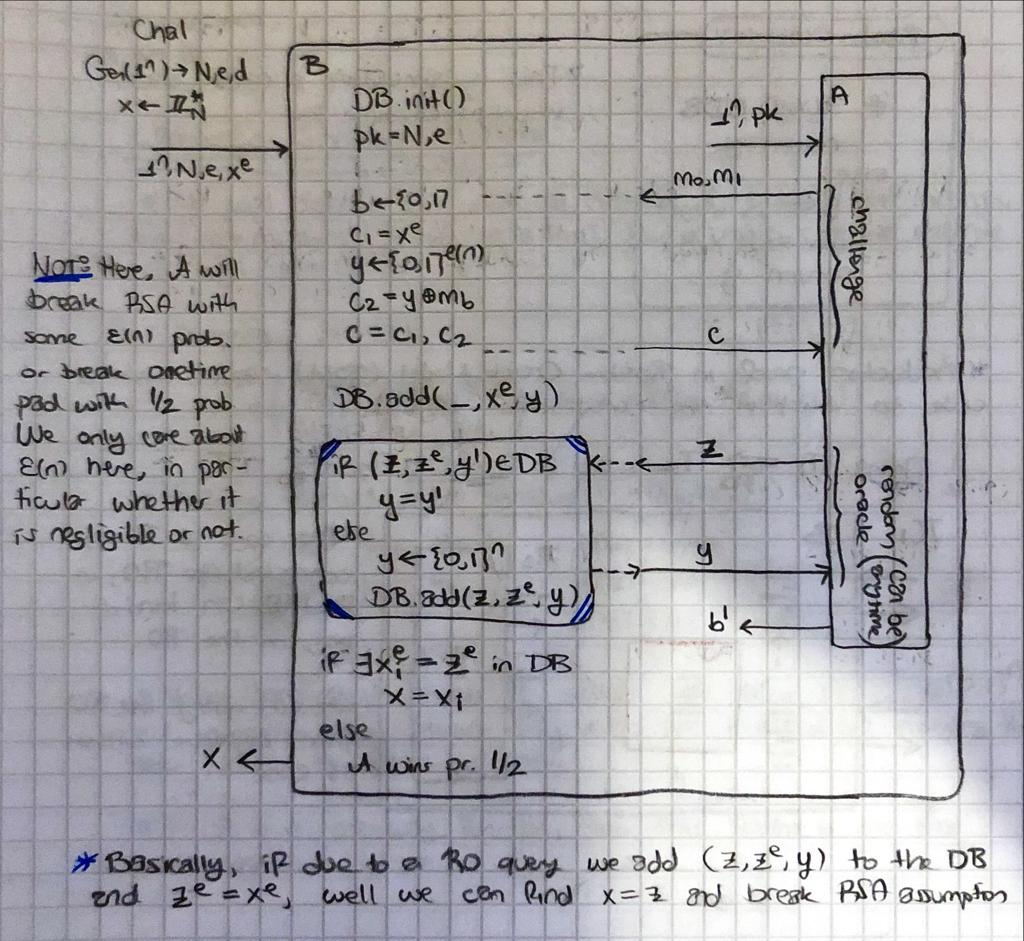
\includegraphics[width=0.9\linewidth]{rsaoracle.jpeg}
\end{figure}


\newpage
\textbf{Q3:} Consider some of the schemes you have seen, try to perform the following replacements to see where the reduction proof fails.
\begin{enumerate}
	\item Replace a random oracle with a PRF
	\item Replace a random oracle with a collision-resistant hash function
	\item Replace a collision-resistant hash function with a second-preimage-resistant hash function
	\item Replace a collision-resistant hash function with a preimage-resistant hash function
\end{enumerate}  

\textbf{A3:} 
First note two things:
\begin{itemize}
	\item If the range of RO is larger than domain, then it is indistinguishable from a PRG.
	\item $F_k(x) = RO(k || x)$ is a PRF using random oracle $RO$.
	\item The success probability of any PPT $\advrs$ in the following experiment is negligible:
	\begin{enumerate}
		\item A random function $H$ is chosen.
		\item $\advrs$ wins if it outputs distinct $x, x'$ with $H(x)=H(x')$.
	\end{enumerate}
	In fact, $\advrs$ succeeds with negligible probability $\mathcal{O}(q^2/2^{l_{out}})$, which is known from the Birthday Problem.
\end{itemize}  

\textit{to do...}
\end{document}